% Imports
\documentclass[9pt, dvipsnames]{beamer}
\usepackage{times}
\usepackage{amsmath}
\usepackage{amsthm}
\usepackage{verbatim}
\usepackage{anyfontsize}
\usepackage{subcaption}
\usepackage{graphicx}
\usepackage[export]{adjustbox}
\usepackage[multidot]{grffile}
\usepackage{tabularx}
\usepackage{tikz}
\usepackage{wasysym}
\usepackage{amsmath,amssymb,amsfonts}

% Beamer Themes
\usetheme{Ilmenau}
\usecolortheme{lily}
\usefonttheme{professionalfonts}
\setbeamertemplate{caption}[numbered]

% Counter
\newcounter{saveenumi}
\resetcounteronoverlays{saveenumi}

% Preamble
\title[DSCI402 Capstone Project]{DSCI402 Capstone Project: Survey of Time Series}
\author{James Craven, Matthew Lindsey, Tina Lane}
\date{December 2024}


\begin{document}


\maketitle

\section{Objectives}
    \begin{frame}{Motivation}
        \begin{enumerate}
            \item Diversify conceptual knowledge \pause
            \item Try different roles in the process \pause
            \item Do something different
        \end{enumerate}
    \end{frame}
    \begin{frame}{Time Series}
        \begin{itemize}
            \item \textbf{Time Series} - a collection of data indexed by time
                as opposed to some other values \pause
            \item \textbf{Time Series Analyses} - a type of regression that attempts
                to capture the correlation of the values w.r.t. time.
        \end{itemize}
    \end{frame}
    \begin{frame}{Project Objectives}
        \begin{enumerate}
            \item Learn about the predominant methods for time series analysis \pause
            \item Analyze the effectiveness of these methods and their pros and
                cons \pause
            \item Create materials to demonstrate our learning
        \end{enumerate}
    \end{frame}
\section{Data Understanding}
    \begin{frame}{The Data}
        A dataset was provided by a local data science company called Delta Bravo. It is an
        anonymized, unclean data set that contains a time series representing semi-aggregate
        motor oil sales data. \pause
        \begin{enumerate}
            \item \textbf{Invoice Date} - the date for which the total sales were recorded
            \item \textbf{Customer Code} - a code that uniquely identifies the customer. These codes
                were anonymized prior to receiving them in order to protect confidentiality
                of the original client.
            \item \textbf{Channel Text} - a label that represented the sales channel. This was almost
                entirely anonymized, and did not reveal any insights.
            \item \textbf{Blend} - The type of oil being sold. A categorical attribute that describing
                whether the oil is conventional or synthetic. This attribute was labelled internally
                as "conventional/synthetic"
            \item \textbf{Variety and Size} - details the oil type and packaging
            \item \textbf{Sale Value} - the target attribute, the total sales recorded for that row
        \end{enumerate}
    \end{frame}
    \begin{frame}{Data Overview}
        \begin{figure}
            \centering
            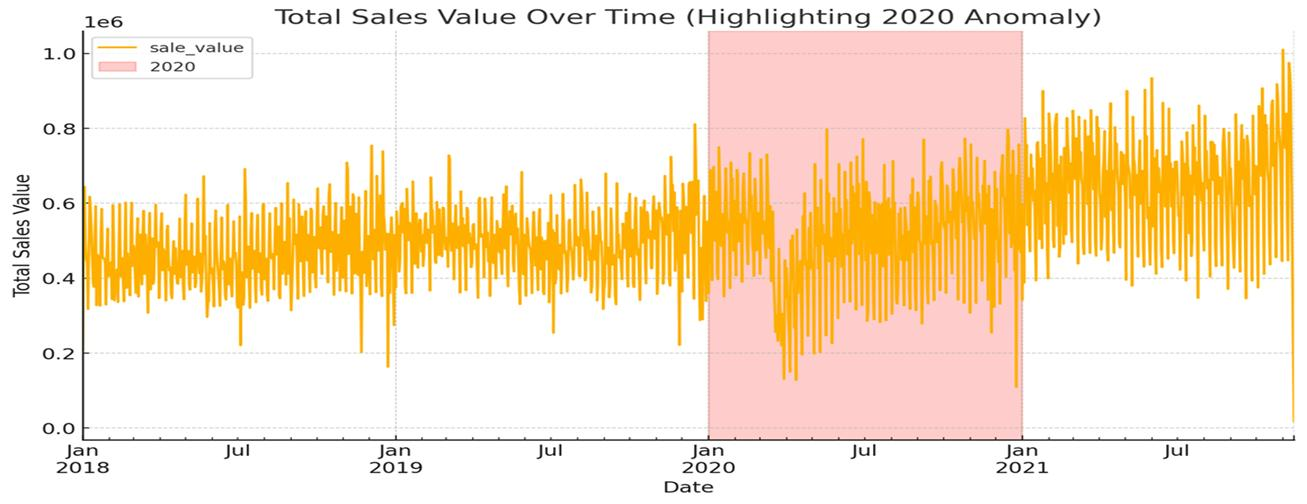
\includegraphics[height=0.42\paperheight]{assets/covid.jpg}
            \label{fig:covid}
        \end{figure}
    \end{frame}
    \begin{frame}{Spread of Locations}
        \begin{figure}
            \centering
            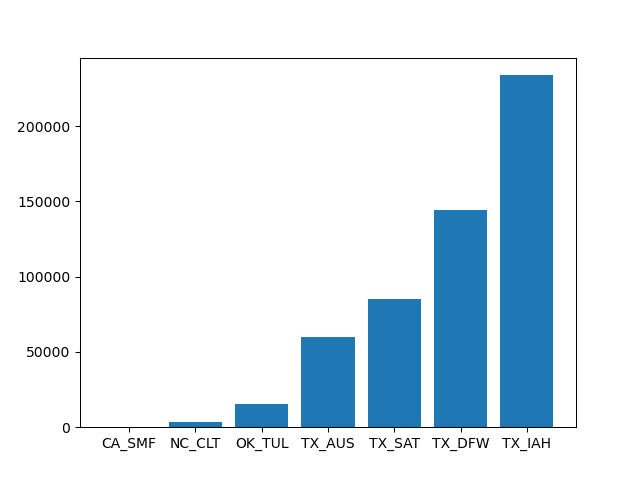
\includegraphics[height=0.6\paperheight]{assets/locations.png}
            \label{fig:location}
        \end{figure}
    \end{frame}
\section{Data Preparation}
    \begin{frame}{Data Selection}
        Of the aforementioned only three were preserved
        \begin{itemize}
            \item \textbf{Invoice Date} - forms the index of the time series \pause
            \item \textbf{Sale Value} - forms the values of the time series \pause
            \item \textbf{Location Code} - allows preservation of regional
                trends
        \end{itemize}
    \end{frame}
    \begin{frame}{Data Cleaning}
        The following steps were taken to handle impurities in the data: \pause
        \begin{itemize}
            \item Negative Values - Removed \pause
            \item Duplicate Values - Aggregated \pause
            \item Missing Values - Filled in and imputed using linear interpolation \pause
            \item Data set split on location
        \end{itemize}
    \end{frame}
\section{Modelling}
    \begin{frame}{Methods Used}
        Two model types were chosen to compare the methods against our data: \pause
        \begin{itemize}
            \item
                Statistical approach: \textbf{ARIMA}
                \begin{itemize}
                    \item Regression based
                    \item Explainable \pause
                \end{itemize}
            \item
                Deep Learning approach: \textbf{Prophet}
                \begin{itemize}
                    \item Neural Net based
                    \item Unexplainable - "black box"
                \end{itemize}
        \end{itemize}
    \end{frame}
    \begin{frame}{Metrics for evaluation}
        The data will be split into training and testing sets to be evaluated based on two metrics \pause
        \begin{itemize}
            \item Root Mean Square Error (RMSE) - measures predictive accuracy by capturing the average 
            magnitude of error \pause
            \item Akaike Information Criterion (AIC) - evaluates the model’s goodness of fit while penalizing 
            complexity
        \end{itemize}
    \end{frame}
    \begin{frame}{Building ARIMA}
        AutoARIMA from the Python module ”pmdarima” automates parameter selection based on optimizing AIC 
        scores.
        \begin{figure}
            \centering
            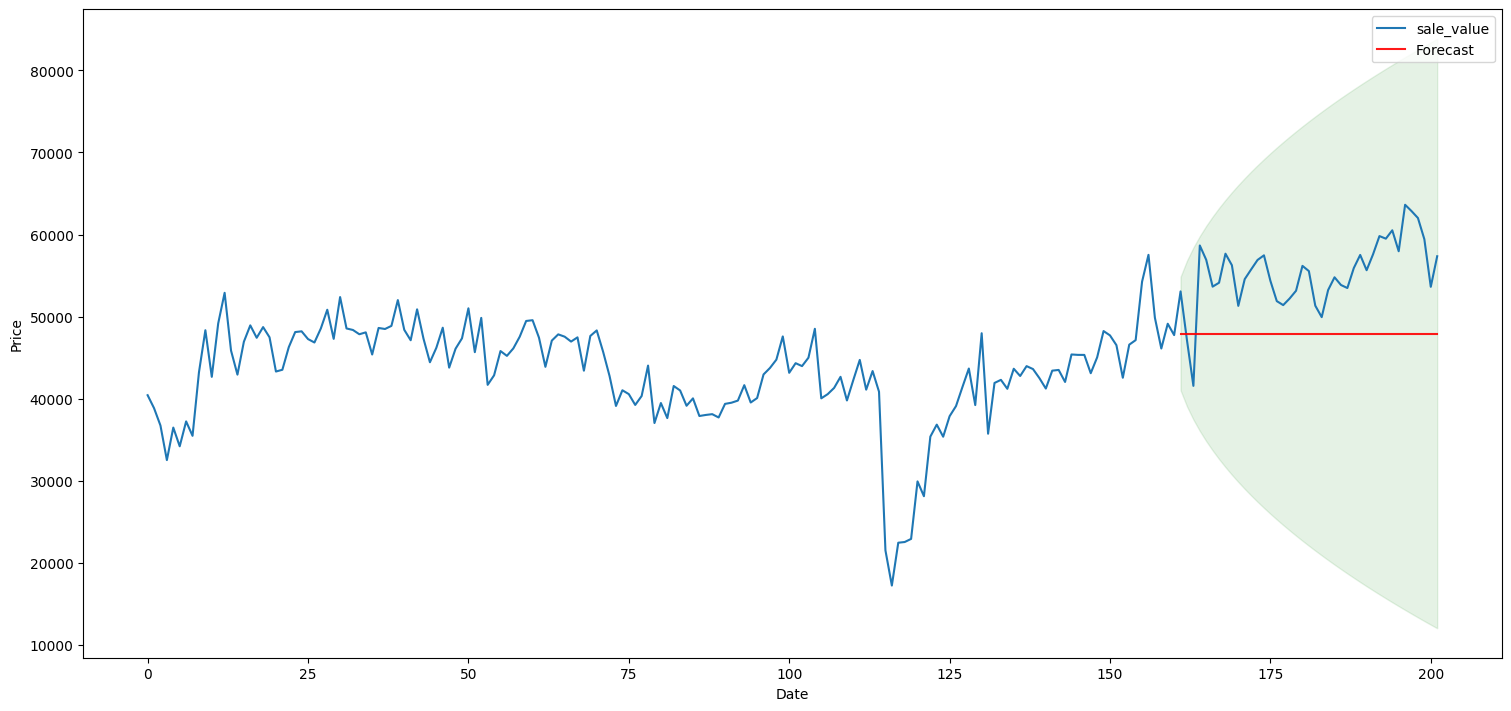
\includegraphics[height=0.47\paperheight]{assets/ARIMA-Weekly.png}
            \label{fig:ARIMA-Weekly}
        \end{figure}
    \end{frame}
    \begin{frame}{Building Prophet}
        After training models without accounting for the COVID-19 lockdowns, we tried to incorporate them as 
        custom one-off holiday periods. Those models took into account the dip in sales in 2020.
        \begin{figure}
            \centering
            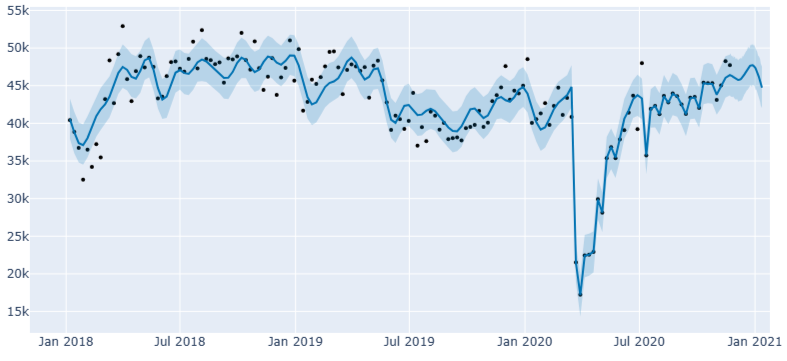
\includegraphics[height=0.47\paperheight]{assets/Prophet-Weekly.png}
            \label{fig:Prophet-Weekly}
        \end{figure}
    \end{frame}
\section{Conclusion}
    \begin{frame}{Model Evaluation}
        \begin{enumerate}
            \item Prophet models that incorporated lockdowns outperformed their counterparts. \pause
            \item ARIMA’s linear approach limited its ability to capture non-linear patterns. \pause
            \item Weekly aggregation helped reduce noise, thus had the lowest AIC and RMSE scores.
        \end{enumerate}
    \end{frame}
    \begin{frame}{ARIMA VS Prophet}
        \begin{figure}
            \centering
            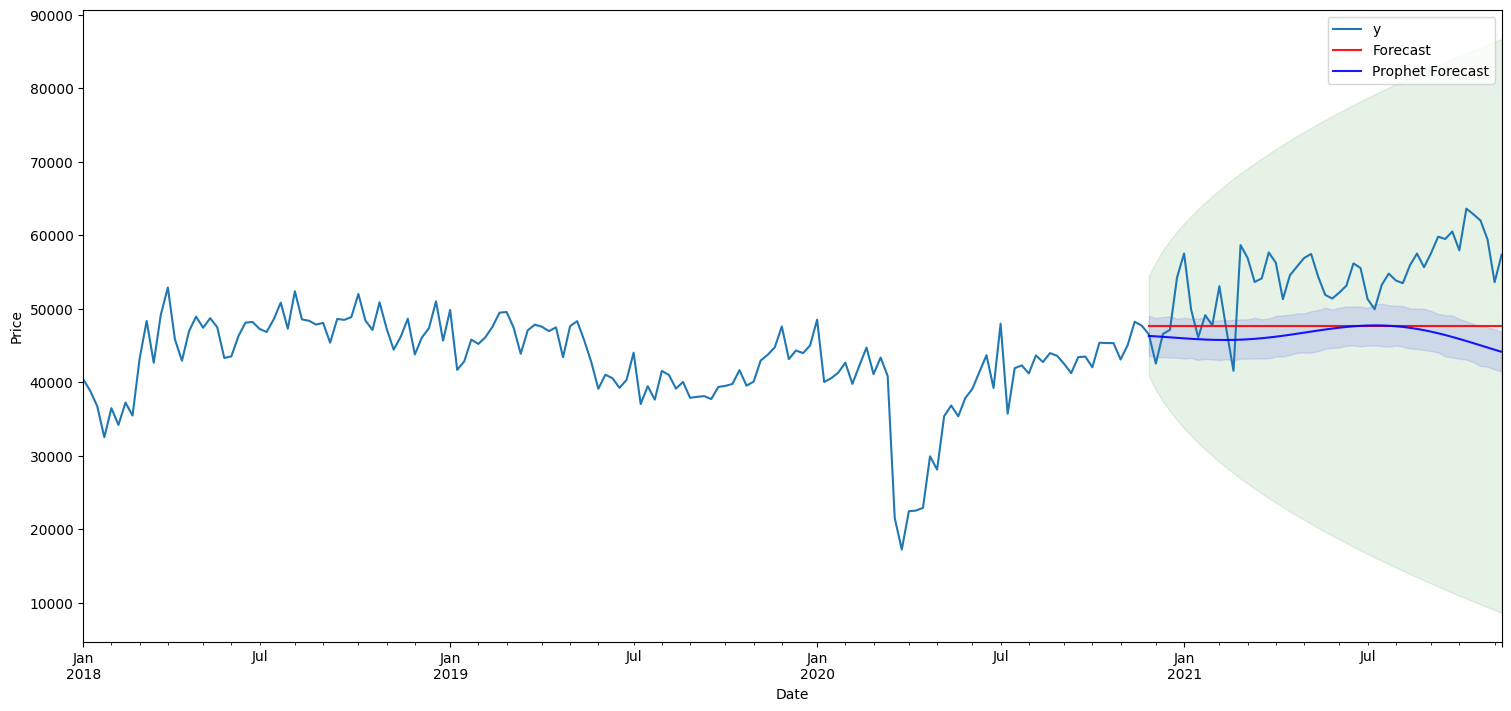
\includegraphics[height=0.47\paperheight]{assets/Model-Comparison.png}
            \label{fig:Model-Comparison}
        \end{figure}
    \end{frame}
    \begin{frame}{Finalized Models}
        The initial test train split was inadequate because the data had a sudden change in trend very close to
        the split date. To ensure model efficacy the models were also trained on just the original test data to 
        see if it could accurately capture the new trend.
        \begin{figure}
            \centering
            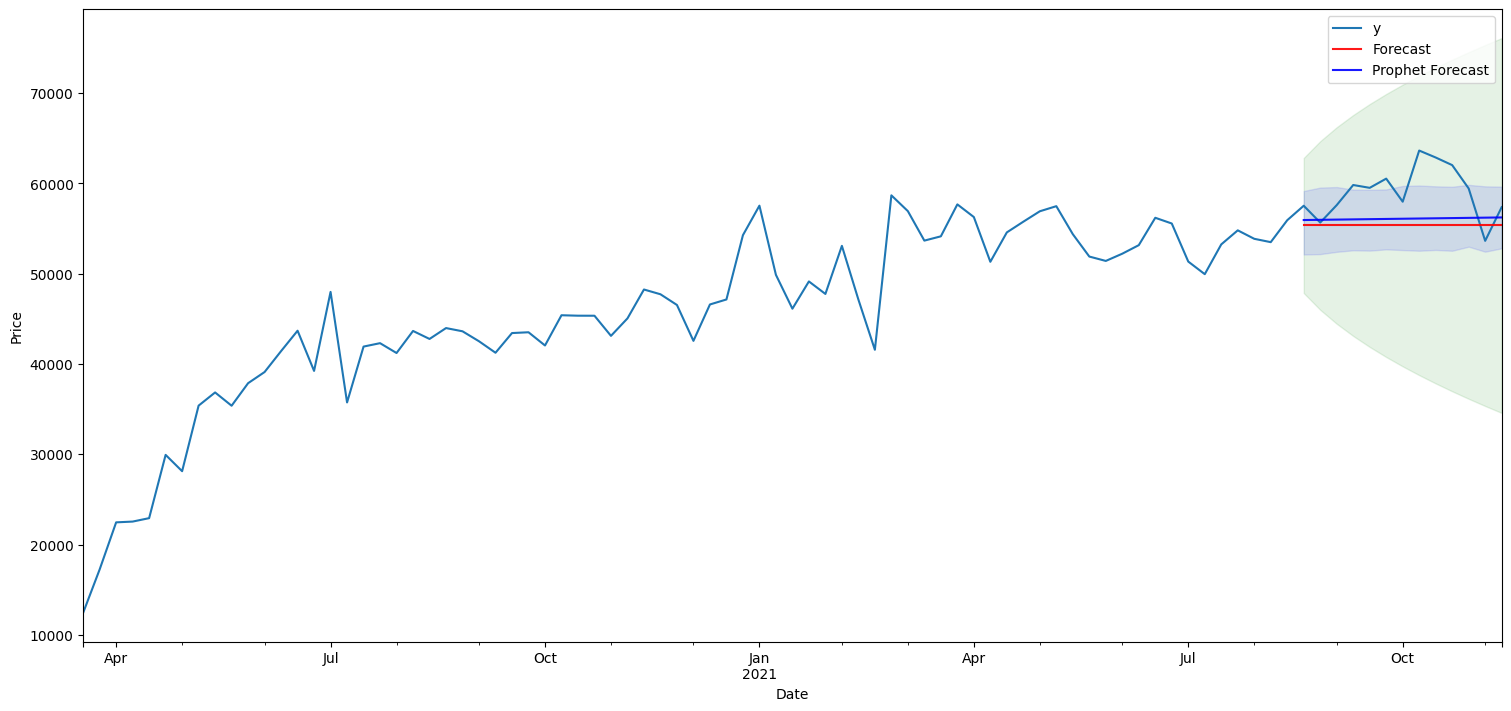
\includegraphics[height=0.47\paperheight]{assets/Model-Comparison-Split.png}
            \label{fig:Model-Comparison-Split}
        \end{figure}
    \end{frame}
    \begin{frame}{Future Action}
        \begin{itemize}
            \item Unused attributes that could be further focused on:
                \begin{itemize}
                    \item Blend
                    \item Size
                    \item Variety \pause
                \end{itemize}
            \item Further research into other models used for time-series data
        \end{itemize}
    \end{frame}
    \begin{frame}{Conclusion}
        \begin{itemize}
            \item The project serves as a survey of both ARIMA and Neural Network based models, and as a 
            comparison of the two. \pause
            \item Both types of models tend to capture similar trends, but with varying levels of granularity 
            and confidence. \pause
            \item ARIMA casts a far wider net, so to speak, and as such values are far more likely to fall in 
            its confidence interval. \pause
            \item Prophet, on the other hand, tends to be more confident in its prediction and can produce a 
            more nuanced forecast. This allows it to capture smaller, temporary noise slightly better as a 
            result.
        \end{itemize}
    \end{frame}

\end{document}